% XeLaTeX document
\documentclass[aspectratio=169, 11pt]{beamer} % для экранов 16:9 оставить

% \documentclass[11pt]{beamer} % для экранов 4:3 оставить

% Редактируем: конфигурация, личные настройки: имя, название предмета и пр. для титульной страницы и метаданных документа здесь



%%% Работа с русским языком
\usepackage[english,russian]{babel}   %% загружает пакет многоязыковой вёрстки
\usepackage{fontspec}      %% подготавливает загрузку шрифтов Open Type, True Type и др.
\defaultfontfeatures{Ligatures={TeX},Renderer=Basic}  %% свойства шрифтов по умолчанию
\setmainfont[Ligatures={TeX,Historic}]{Times New Roman} %% задаёт основной шрифт документа
\setsansfont{Comic Sans MS}                    %% задаёт шрифт без засечек
\setmonofont{Courier New}

%%%% Работа с русским языком
\usepackage[english,russian]{babel}   %% загружает пакет многоязыковой вёрстки
\usepackage{fontspec}      %% подготавливает загрузку шрифтов Open Type, True Type и др.
\defaultfontfeatures{Ligatures={TeX},Renderer=Basic}  %% свойства шрифтов по умолчанию
\setmainfont[Ligatures={TeX,Historic}]{Times New Roman} %% задаёт основной шрифт документа
\setsansfont{Comic Sans MS}                    %% задаёт шрифт без засечек
\setmonofont{Courier New}
\usepackage{indentfirst}
\frenchspacing

\renewcommand{\epsilon}{\ensuremath{\varepsilon}}
\renewcommand{\phi}{\ensuremath{\varphi}}
\renewcommand{\kappa}{\ensuremath{\varkappa}}
\renewcommand{\le}{\ensuremath{\leqslant}}
\renewcommand{\leq}{\ensuremath{\leqslant}}
\renewcommand{\ge}{\ensuremath{\geqslant}}
\renewcommand{\geq}{\ensuremath{\geqslant}}
\renewcommand{\emptyset}{\varnothing}

%%% Дополнительная работа с математикой
\usepackage{amsmath,amsfonts,amssymb,amsthm,mathtools} % AMS
\usepackage{icomma} % "Умная" запятая: $0,2$ --- число, $0, 2$ --- перечисление

%% Номера формул
%\mathtoolsset{showonlyrefs=true} % Показывать номера только у тех формул, на которые есть \eqref{} в тексте.
%\usepackage{leqno} % Нумерация формул слева

%% Свои команды
\DeclareMathOperator{\sgn}{\mathop{sgn}}

%% Перенос знаков в формулах (по Львовскому)
\newcommand*{\hm}[1]{#1\nobreak\discretionary{}
	{\hbox{$\mathsurround=0pt #1$}}{}}

%%% Работа с картинками
\usepackage{graphicx}  % Для вставки рисунков
\graphicspath{{images/}{images2/}}  % папки с картинками
\setlength\fboxsep{3pt} % Отступ рамки \fbox{} от рисунка
\setlength\fboxrule{1pt} % Толщина линий рамки \fbox{}
\usepackage{wrapfig} % Обтекание рисунков текстом

%%% Работа с таблицами
\usepackage{array,tabularx,tabulary,booktabs} % Дополнительная работа с таблицами
\usepackage{longtable}  % Длинные таблицы
\usepackage{multirow} % Слияние строк в таблице


%%% Программирование
\usepackage{etoolbox} % логические операторы


%%% Страница
\usepackage{extsizes} % Возможность сделать 14-й шрифт
\usepackage{geometry} % Простой способ задавать поля
\geometry{top=25mm}
\geometry{bottom=35mm}
\geometry{left=35mm}
\geometry{right=20mm}
%
%\usepackage{fancyhdr} % Колонтитулы
% 	\pagestyle{fancy}
%\renewcommand{\headrulewidth}{0pt}  % Толщина линейки, отчеркивающей верхний колонтитул
% 	\lfoot{Нижний левый}
% 	\rfoot{Нижний правый}
% 	\rhead{Верхний правый}
% 	\chead{Верхний в центре}
% 	\lhead{Верхний левый}
%	\cfoot{Нижний в центре} % По умолчанию здесь номер страницы

\usepackage{setspace} % Интерлиньяж
%\onehalfspacing % Интерлиньяж 1.5
%\doublespacing % Интерлиньяж 2
%\singlespacing % Интерлиньяж 1

\usepackage{lastpage} % Узнать, сколько всего страниц в документе.

\usepackage{soul} % Модификаторы начертания

\usepackage{hyperref}
\usepackage[usenames,dvipsnames,svgnames,table,rgb]{xcolor}
\hypersetup{				% Гиперссылки
	unicode=true,           % русские буквы в раздела PDF
	pdftitle={Заголовок},   % Заголовок
	pdfauthor={Автор},      % Автор
	pdfsubject={Тема},      % Тема
	pdfcreator={Создатель}, % Создатель
	pdfproducer={Производитель}, % Производитель
	pdfkeywords={keyword1} {key2} {key3}, % Ключевые слова
	colorlinks=true,       	% false: ссылки в рамках; true: цветные ссылки
	linkcolor=red,          % внутренние ссылки
	citecolor=black,        % на библиографию
	filecolor=magenta,      % на файлы
	urlcolor=cyan           % на URL
}

\usepackage{csquotes} % Еще инструменты для ссылок

%\usepackage[style=authoryear,maxcitenames=2,backend=biber,sorting=nty]{biblatex}

\usepackage{multicol} % Несколько колонок

\usepackage{tikz} % Работа с графикой
\usepackage{pgfplots}
\usepackage{pgfplotstable}




% рабочие ссылки в документе
\usepackage{hyperref}
\urlstyle{same}
% графика
\usepackage{graphicx}
\usepackage{tikz}
%\usepackage{pgfplots}

% качественные листинги кода
%\usepackage{minted}
%\usepackage{listings}
%\usepackage{lstfiracode}


% библиография
\bibliographystyle{templates/gost-numeric.bbx}
\usepackage{csquotes}
\usepackage[parentracker=true,backend=biber,hyperref=true,bibencoding=utf8,style=numeric-comp,language=auto,autolang=other,citestyle=gost-numeric,defernumbers=true,bibstyle=gost-numeric,sorting=ntvy]{biblatex}

% для заголовков
\usepackage{caption} 

% разное для математики
\usepackage{amsmath, amsfonts, amssymb, amsthm, mathtools}

% водяной знак на документе, см. main.tex
%\usepackage[printwatermark]{xwatermark} 

% для презентаций
\usepackage{here}
\usepackage{animate}
\usepackage{bm}


\newcommand{\university}{РГУ нефти и газа имени И.М.Губкина}
\newcommand{\faculty}{кафедра РиЭНМ}
\newcommand{\department}{департамент}
\newcommand{\city}{Москва}
\newcommand{\num}{ № 1}
\newcommand{\docname}{Исследование скважин и пластов. Введение}
\newcommand{\tutorname}{Хабибуллин Р.А.}
\newcommand{\studentname}{студент}
\newcommand{\group}{группы нет}

% настройка метаданных документа
\institute[\university]{\university \\ \faculty}
\title[\docname]{Лекция 3. Исследования на стационарных режимах работы}
\author[\tutorname]{\small  \tutorname}
\date{\the\year} 

\makeatletter
\setbeamertemplate{title page}{
	\begin{minipage}[b][\paperheight]{\textwidth}
		\centering
		\ifx\insertinstitute\@empty\else\usebeamertemplate*{institute}\fi
		\vfill
		\ifx\inserttitle\@empty\else\usebeamertemplate*{title}\fi
		\vfill
		\usebeamertemplate*{title separator}
		\ifx\beamer@shortauthor\@empty\else\usebeamertemplate*{author}\fi
		\ifx\insertdate\@empty\else\usebeamertemplate*{date}\fi
		\vfill
		\vspace*{1mm}
	\end{minipage}
}


% ---------------------------------------------------------------------------------------------
\begin{document}

\begin{frame}
	\titlepage
\end{frame}
% ---------------------------------------------------------------------------------------------
\begin{frame}{Содержание лекции}
	\begin{enumerate}
		\item Идея исследований на стационарном режиме работы
		\item Индикаторная диаграмма IPR
		\item Построение IPR на основе стационарного решения
		\item Построение IPR на основе нестационарного решения
		\item Построение IPR на основе численного решения
	\end{enumerate}

\end{frame}

% ---------------------------------------------------------------------------------------------
\begin{frame}{Идея исследований на стационарном режиме работы}

Если при эксплуатации скважины стационарный режим доминирует, то можно восстановив его характеристику обеспечить управление скважиной

\begin{figure}[h!]
	\begin{center}
		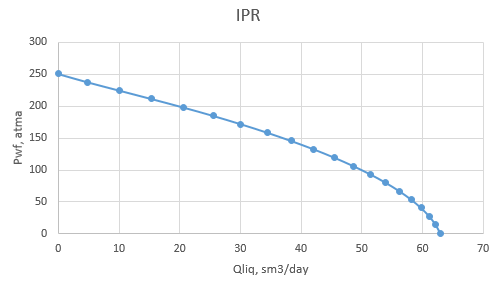
\includegraphics[width=7cm]{pics/ipr_1.png}
		%\caption{Индикаторная диаграмма}
		\label{ris:ipr_1}
	\end{center}
\end{figure}

Задача исследования - восстановить IPR
	
\end{frame}
% ---------------------------------------------------------------------------------------------
\begin{frame}{Индикаторная диаграмма IPR}
	
	IPR - ключевая характеристика стационарного режима работы скважины
	
	\begin{figure}[h!]
		\begin{center}
			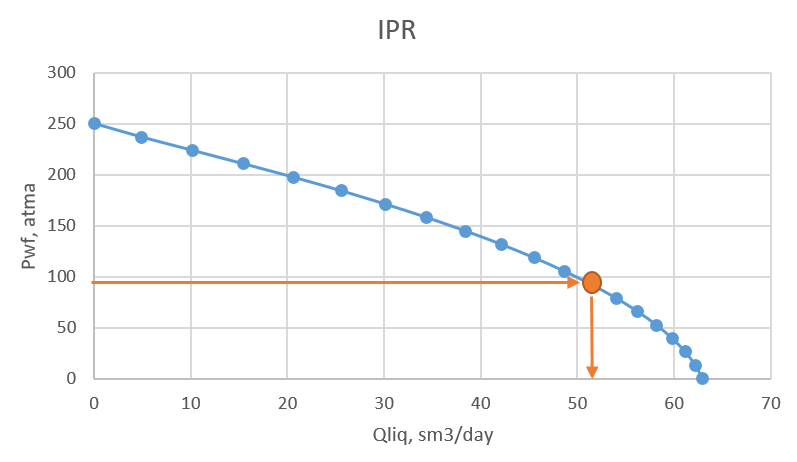
\includegraphics[width=9cm]{pics/ipr_2.png}
			%\caption{Индикаторная диаграмма}
			\label{ris:ipr_1}
		\end{center}
	\end{figure}
	
	Позволяет определить прогнозный дебит скважины при изменении забойного давления
	
\end{frame}

% ---------------------------------------------------------------------------------------------
\begin{frame}{Распространенные модели IPR}
	
	\begin{itemize}
		\item Закон Дарси
		\item Закон Дарси с поправкой Вогеля (композитная кривая Вогеля)
		\item Другие подходы
	\end{itemize}
	
	\begin{figure}[h!]
		\begin{center}
			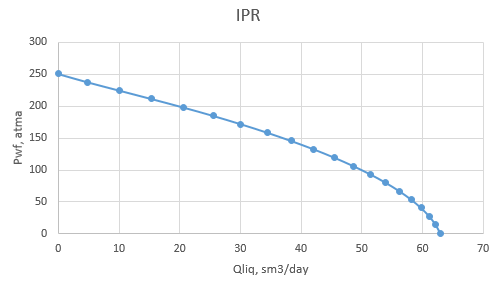
\includegraphics[width=7cm]{pics/ipr_1.png}
			%\caption{Индикаторная диаграмма}
			\label{ris:ipr_1}
		\end{center}
	\end{figure}
	
\end{frame}

% ---------------------------------------------------------------------------------------------
\begin{frame}{Задачи}
	
	\begin{enumerate}
		\item Постройте IPR Вогеля с использованием unifloc VBA
		\item Постройте IPR с использованием нестационарного решения линейного стока
		\item Постройте IPR с использованием ГДМ для различных конфигураций
	\end{enumerate}
	

	
\end{frame}


% Не редактируем: Страница библиографии (формируется автоматически из книжек, указанных в refs.bib и пометок \cite{имя_источника} в тексте)
%\include{templates/bib-page}

\end{document}
